\documentclass{beamer}
\usepackage[utf8]{inputenc}   % pour pouvoir taper les accents directement     
\usepackage{amsfonts,amssymb,amsmath}
\usepackage{tikz}
\usepackage{array}
\usetikzlibrary{patterns}
\usepackage[absolute,showboxes,overlay]{textpos}     
\textblockorigin{0pt}{0pt}                          
\TPshowboxesfalse  
 \usepackage{lmodern,multido}

\newcommand{\R}{\mathbb{R}}
\newcommand{\C}{\mathbb{C}}
\newcommand{\Z}{\mathbb{Z}}
\newcommand{\N}{\mathbb{N}}
\newcommand{\Q}{\mathbb{Q}}
\newcommand{\E}{(-4,-1) rectangle (4,4)}
\newcommand{\A}{(0,0) ++(135:2) circle (2)}
\newcommand{\B}{(0,0) ++(45:2) circle (2)}

\begin{document}
 \addtobeamertemplate{navigation symbols}{}{\hspace{1em} \usebeamerfont{footline}%
    \insertframenumber/\inserttotalframenumber }

 %%%%%%%%%%%%%%%%%%%%%%%%%%%%%%%%%%%%%%%%%%%%%%%%%%%%%%%%%%%%%%%

\begin{frame}{Introduction aux statistiques}{}

\begin{center}{\bf \Large Informations générales 2024-2025} \end{center}
\vspace{0.2cm}

\begin{itemize}
\item \large Objectifs : 
\begin{itemize}
\item Rappels sur les probabilités et les variables aléatoires discrètes
\item Variables aléatoires et lois usuelles continues
\item Introduction à la théorie de l'estimation 
\item Tests statistiques
%\item {\it ANOVA et tests non paramétriques non traités} \\
\end{itemize}

%\item parfois simplifié


\item Evaluation : 
\begin{itemize}
\item 2 CC sous forme de QCM ($30\%$) + 1 examen final ($70\%$) \\
\end{itemize}

\item Documents à votre disposition : 
\begin{itemize}
\item distribués en TD : formulaire de cours (autorisé à l'examen) + feuilles de TD
\item sur Moodle : diapos + polycopié de cours + corrigés de certains exercices + archives d'examens 
\end{itemize}
\end{itemize}

\end{frame}

%%%%%%%%%%%%%%%%%%%%%%%%%%%%%%%%%%%%%%%%%%%%%

\begin{frame}{Rappels de probabilité}

\begin{itemize}
\item Expérience aléatoire 
\begin{itemize}
\item préciser tous les résultats possibles
\item attribuer, à chaque résultat, un poids = probabilité
\end{itemize}
\item $\Omega$ = l'ensemble des résultats possibles d'une expérience
aléatoire
\item événement certain (fini ou infini)= $ \Omega$ 
\item événement élémentaire = $\{\omega\}, \omega\in \Omega$
\item événement = partie de $\Omega$ (plusieurs évènements élémentaires)
\item événement impossible= $\emptyset$
\end{itemize}

\end{frame}

%%%%%%%%%%%%%%%%%%%%%%%%%%%%%%%%%%%%%%%%%%%%%%%

\begin{frame}{Rappels de probabilité}

\begin{tabular}{m{7cm}>{\centering\arraybackslash}m{3cm}}
 Si $A\subset\Omega$ et $B\subset\Omega$& 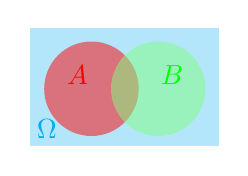
\begin{tikzpicture}[scale=0.3]
\fill[color=cyan!30] \E;
\fill[opacity=0.5,red] \A;
\fill[opacity=0.5,color=green!50] \B;
\draw[color=cyan] (-3.3,-0.3)node{$\Omega$} ;
\draw[color=red] (-2,2)node{$A$} ;
\draw[color=green] (2,2)node{$B$} ;
\end{tikzpicture}\\
alors \\
$A\cup B$ :  $A$ {\bf ou} $B$ est réalisé & 
\begin{tikzpicture}[scale=0.2]
\fill[color=cyan!30] \E;
\fill[blue] \A;
\fill[blue] \B;
\end{tikzpicture}\\
\\
 $A\cap B$ : les événements $A$ {\bf et} $B$ sont réalisés & 
 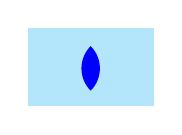
\begin{tikzpicture}[scale=0.2]
\fill[color=cyan!30] \E;
\begin{scope}
\clip \B;
\fill[blue] \A;
\end{scope}
\end{tikzpicture}
\\
\\
 $\overline{A}$ ; l'événement $A$  {\bf n'est pas} réalisé&
 
\begin{tikzpicture}[scale=0.2]
\fill[blue] \E;
\fill[color=cyan!30] \A;

\end{tikzpicture}
\\
\end{tabular}


\end{frame}

%%%%%%%%%%%%%%%%%%%%%%%%%

\begin{frame}{Rappels de probabilité}


Une \textcolor{red}{probabilité} sur $\Omega$ est une application $Pr:\Omega \longrightarrow [0,1]$ telle que

\begin{itemize}
\begin{tabular}{m{7cm}>{\centering\arraybackslash}m{3cm}}
\item $Pr(\emptyset) = 0$\\
\item $Pr(\Omega) = 1 $\\ 
\item $A \cap B = \emptyset\Longrightarrow Pr(A \cup B) = Pr(A)+Pr(B)$
\\
\end{tabular}
\end{itemize}

On a les propriétés :

\begin{itemize}
\begin{tabular}{m{7cm}>{\centering\arraybackslash}m{3cm}}
\item $A \subset B \Longrightarrow Pr(A) \leq Pr(B)$& 
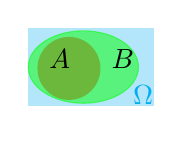
\begin{tikzpicture}[scale=0.2]
\fill[color=cyan!30] \E;
\fill[opacity=0.5,red] \A;
\draw[color=cyan] (3.3,-0.3)node{$\Omega$} ;
\draw[opacity=0.5,fill=green,color=green] (-0.5,1.5) circle (3.5 and 2.3);
\draw (-2,2)node{$A$} ;
\draw (2,2)node{$B$} ;
\end{tikzpicture}
\\
\item $Pr(\overline{A}) = 1-Pr(A)$ 
 & 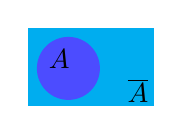
\begin{tikzpicture}[scale=0.2]
\fill[color=cyan] \E;
\fill[blue!70] \A;
\draw (3,0)node{$\overline{A}$} ;
\draw (-2,2)node{$A$} ;
\end{tikzpicture}
\\
 \item $Pr(A) = Pr(A \cap B) + Pr(A \cap \overline{B})$  &
 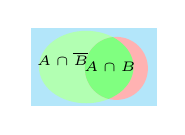
\begin{tikzpicture}[scale=0.2]
\fill[color=cyan!30] \E;
\fill[color=green!30] (-0.5,1.5) circle (3 and 2.3);;
\fill[color=red!30] \B;
\begin{scope}
\clip \B;
\fill[green!50] (-0.5,1.5) circle (3 and 2.3);;
\end{scope}
\draw (-2,2)node{\tiny $A \cap \overline B$} ;
\draw (1,1.5)node{\tiny $A \cap  B$} ;
\end{tikzpicture}
\\
 \item $Pr(A\cup B) = Pr(A) + Pr(B) - Pr(A \cap B)$ 
&
 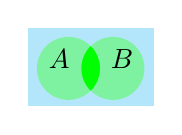
\begin{tikzpicture}[scale=0.2]
\fill[color=cyan!30] \E;
\fill[opacity=0.5,green!70] \A;
\fill[opacity=0.5,green!70] \B;
\begin{scope}
\clip \B;
\fill[green] \A;
\end{scope}
\draw (-2,2)node{$A$} ;
\draw (2,2)node{$B$} ;
\end{tikzpicture}
\\

\end{tabular}
\end{itemize}

\end{frame}


%%%%%%%%%%%%%%%%%

\begin{frame}{Rappels de probabilité}

\begin{itemize}
\item $A$ et $B$ sont \textcolor{red}{ indépendants} si $Pr(A\cap B)=Pr(A)\times Pr(B)$

\
\item Si $\Omega$ fini et tous les événements élémentaires ont la même
probabilité ($1/card(\Omega)$)  alors, pour tout  $A\subset \Omega$ :
$$
Pr(A)=\frac{card(A)}{card(\Omega)}=\frac{nombre\, de\,  cas\, favorables}{nombre \, de \, cas\, possibles}\,
$$
\end{itemize}

\end{frame}

%%%%%%%%%%%%%%%%%

\begin{frame}{Rappels de probabilité}

  La \textcolor{red}{probabilité conditionnelle} de $A$ {\bf sachant} $B$ est
définie par:
$$
Pr(A|B)=\frac{Pr(A\cap B)}{Pr(B)}
$$

\begin{center}
\begin{tabular}{m{3.5cm} m{0.3cm}m{3.5cm}}
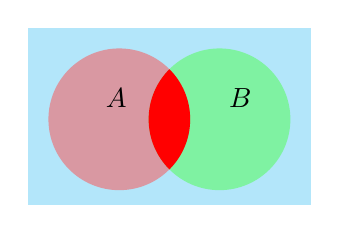
\begin{tikzpicture}[scale=0.45]
\fill[color=cyan!30] \E;
\fill[opacity=0.5,red!70] \A;
\fill[opacity=0.5,green!70] \B;
\begin{scope}
\clip \B;
\fill[red] \A;
\end{scope}
\draw (-1.5,2)node{$A$} ;
\draw (2,2)node{$B$} ;
\end{tikzpicture}
&$\rightarrow$&
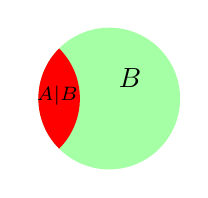
\begin{tikzpicture}[scale=0.45]
\fill[opacity=0.5,green!70] \B;
\begin{scope}
\clip \B;
\fill[red] \A;
\end{scope}
\draw (-0.05,1.5)node{\scriptsize {$ A|B$}} ;
\draw (2,2)node{$B$} ;
\end{tikzpicture}
\end{tabular}
\end{center}

\end{frame}

 %%%%%%%%%%%%%%%%%%%%%%%%%%%%%%%%%%%%%%%%%%%%%%%%%%%%%%%%%%%%%%%
\begin{frame}{Rappels de probabilité}
\begin{textblock*}{\textwidth}(7cm,2cm)

%\only<1>
  { %\begin{center}
\begin{tabular}{m{1.5cm} m{0.3cm}m{1.5cm}}
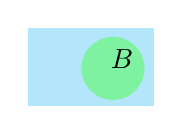
\begin{tikzpicture}[scale=0.2]
\fill[color=cyan!30] \E;
\fill[opacity=0.5,green!70] \B;
\draw (2,2)node{$B$} ;
\end{tikzpicture}
&$\rightarrow$&
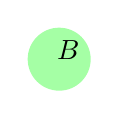
\begin{tikzpicture}[scale=0.2]
\fill[opacity=0.5,green!70] \B;
\draw (2,2)node{$B$} ;
\end{tikzpicture}
\end{tabular}
%\end{center}
}

%\only<2>
  {  %\begin{center}
\begin{tabular}{m{1.5cm} m{0.6cm}m{1.5cm}}
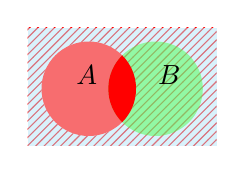
\begin{tikzpicture}[scale=0.3]
\fill[pattern color=red,pattern=north east lines,] \E;
\fill[white] \A;
\fill[opacity=0.5,color=cyan!30] \E;
\fill[opacity=0.8,red!70] \A;
\fill[opacity=0.5,green!70] \B;
\begin{scope}
\clip \B;
\fill[red] \A;
\end{scope}
\draw (-1.5,2)node{$A$} ;
\draw (2,2)node{$B$} ;
\end{tikzpicture}
&$\;\;\;\;\;\; \rightarrow$&
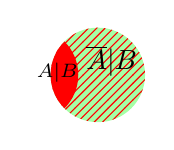
\begin{tikzpicture}[scale=0.3]
\fill[opacity=0.5,green!70] \B;
\begin{scope}
\clip \B;
\fill[pattern color=red,pattern=north east lines,] \E;
\fill[red] \A;
\end{scope}
\draw (-0.3,1.5) node{\scriptsize {$A|B$}} ;
\draw (2,2) node{$\overline{A}|B$} ;
\end{tikzpicture}
\end{tabular}
%\end{center}
}



%\only<3>
  {%\begin{center}
\begin{tabular}{m{1.5cm} m{0.3cm}m{1.5cm}}
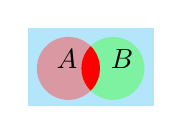
\begin{tikzpicture}[scale=0.2]
\fill[color=cyan!30] \E;
\fill[opacity=0.5,red!70] \A;
\fill[opacity=0.5,green!70] \B;
\begin{scope}
\clip \B;
\fill[red] \A;
\end{scope}
\draw (-1.5,2)node{$A$} ;
\draw (2,2)node{$B$} ;
\end{tikzpicture}
&$\rightarrow$&
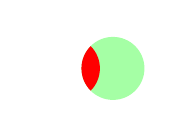
\begin{tikzpicture}[scale=0.2]
\fill[color=white] \E;
\fill[opacity=0.5,green!70] \B;
\begin{scope}
\clip \B;
\fill[red] \A;
\end{scope}
\end{tikzpicture}\\
&$\searrow$&\\
&&
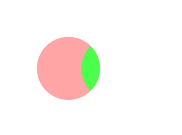
\begin{tikzpicture}[scale=0.2]
\fill[color=white] \E;
\fill[opacity=0.5,red!70] \A;
\begin{scope}
\clip  \A;
\fill[green!70]\B;
\end{scope}
\end{tikzpicture}
\end{tabular}
%\end{center}
}

\end{textblock*}

\begin{textblock*}{8cm}(1cm,5cm)
On a les propriétés
\begin{itemize}
\item $Pr(B|B)=1$ 
\item $Pr(A|B)+Pr(\overline{A}|B)=1$ 
\item ${\displaystyle Pr(B|A)= \frac{Pr(B)}{Pr(A)}.Pr(A|B)}$ 
\item $A$ et $B$ sont indépendants si et seulement si $Pr(A|B)=P(A)$ 
\end{itemize}
\end{textblock*}


\end{frame}
%*****************



\begin{frame}{Rappels de probabilité}

\noindent  {\bf La formule des probabilités totales} :


\begin{center}
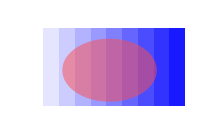
\begin{tikzpicture}[scale=0.2]
\draw (2,2)node{$B$} ;
\multido{\i=0+10}{10}{%
\fill[color=blue!\i] (-4+\i/10,-1) rectangle (-3+\i/10,4);}
\fill[opacity=0.5,red!70] (1.2,1.3) ellipse  (3 and 2);
\end{tikzpicture}
\end{center}


Si $(B_1, B_2, \hdots, B_k)$ forme une partition de $\Omega$  alors on a
$$
Pr(A)=Pr(A \cap B_1) + Pr(A \cap B_2) + \hdots + Pr(A \cap B_k) 
$$
$$
=Pr(A|B_1).Pr(B_1)+ Pr(A|B_2).Pr(B_2) + \hdots + Pr(A|B_k).Pr(B_k)
$$

\noindent Cas particulier : 
${\displaystyle Pr(A)=  Pr(A \cap B)+Pr(A \cap \overline{B})
=  Pr(A|B).Pr(B)+Pr(A| \overline{B}). Pr(\overline{B})}$
\end{frame}

\end{document}









\\

 







